\subsection{Problem definition}
\subsubsection*{System's variable}
\begin{itemize}
    \item Reference path $\pi$, $\pi : \mathbb{R} \longrightarrow \mathbb{R}^3, \quad \pi(s_\pi) = (x_\pi, y_\pi,\theta_\pi)$
    \item Distance $s$ : $s \in \mathbb{R}$, distance along the path corresponding to the vehicle’s position projections.
    \item Lateral error $d$ : $d \in \mathbb{R},\quad d = ||P_r - P_{r,\pi}||$, distance between the path and the vehicle.
    \item heading error $s$ : $\theta_e \in \mathbb{R}, \quad \theta_e = (\theta - \theta_\pi)$, difference between vehicle yaw angle and path's orientation.
    \item Longitudinal speed $v$ : $v \in \mathbb{R}^+$
    \item Longitudinal speed reference $v_{ref}$ : $v_{ref} \in \mathbb{R}^+$
    \item Steering wheel position $\phi$ : $\phi \in \mathbb{R}$
    \item Steering wheel reference $\phi_{ref}$ : $\phi_{ref} \in [-4\pi,4\pi]$
    \item Path's curvature $\kappa$
\end{itemize}

\begin{figure}[H]
    \centering
    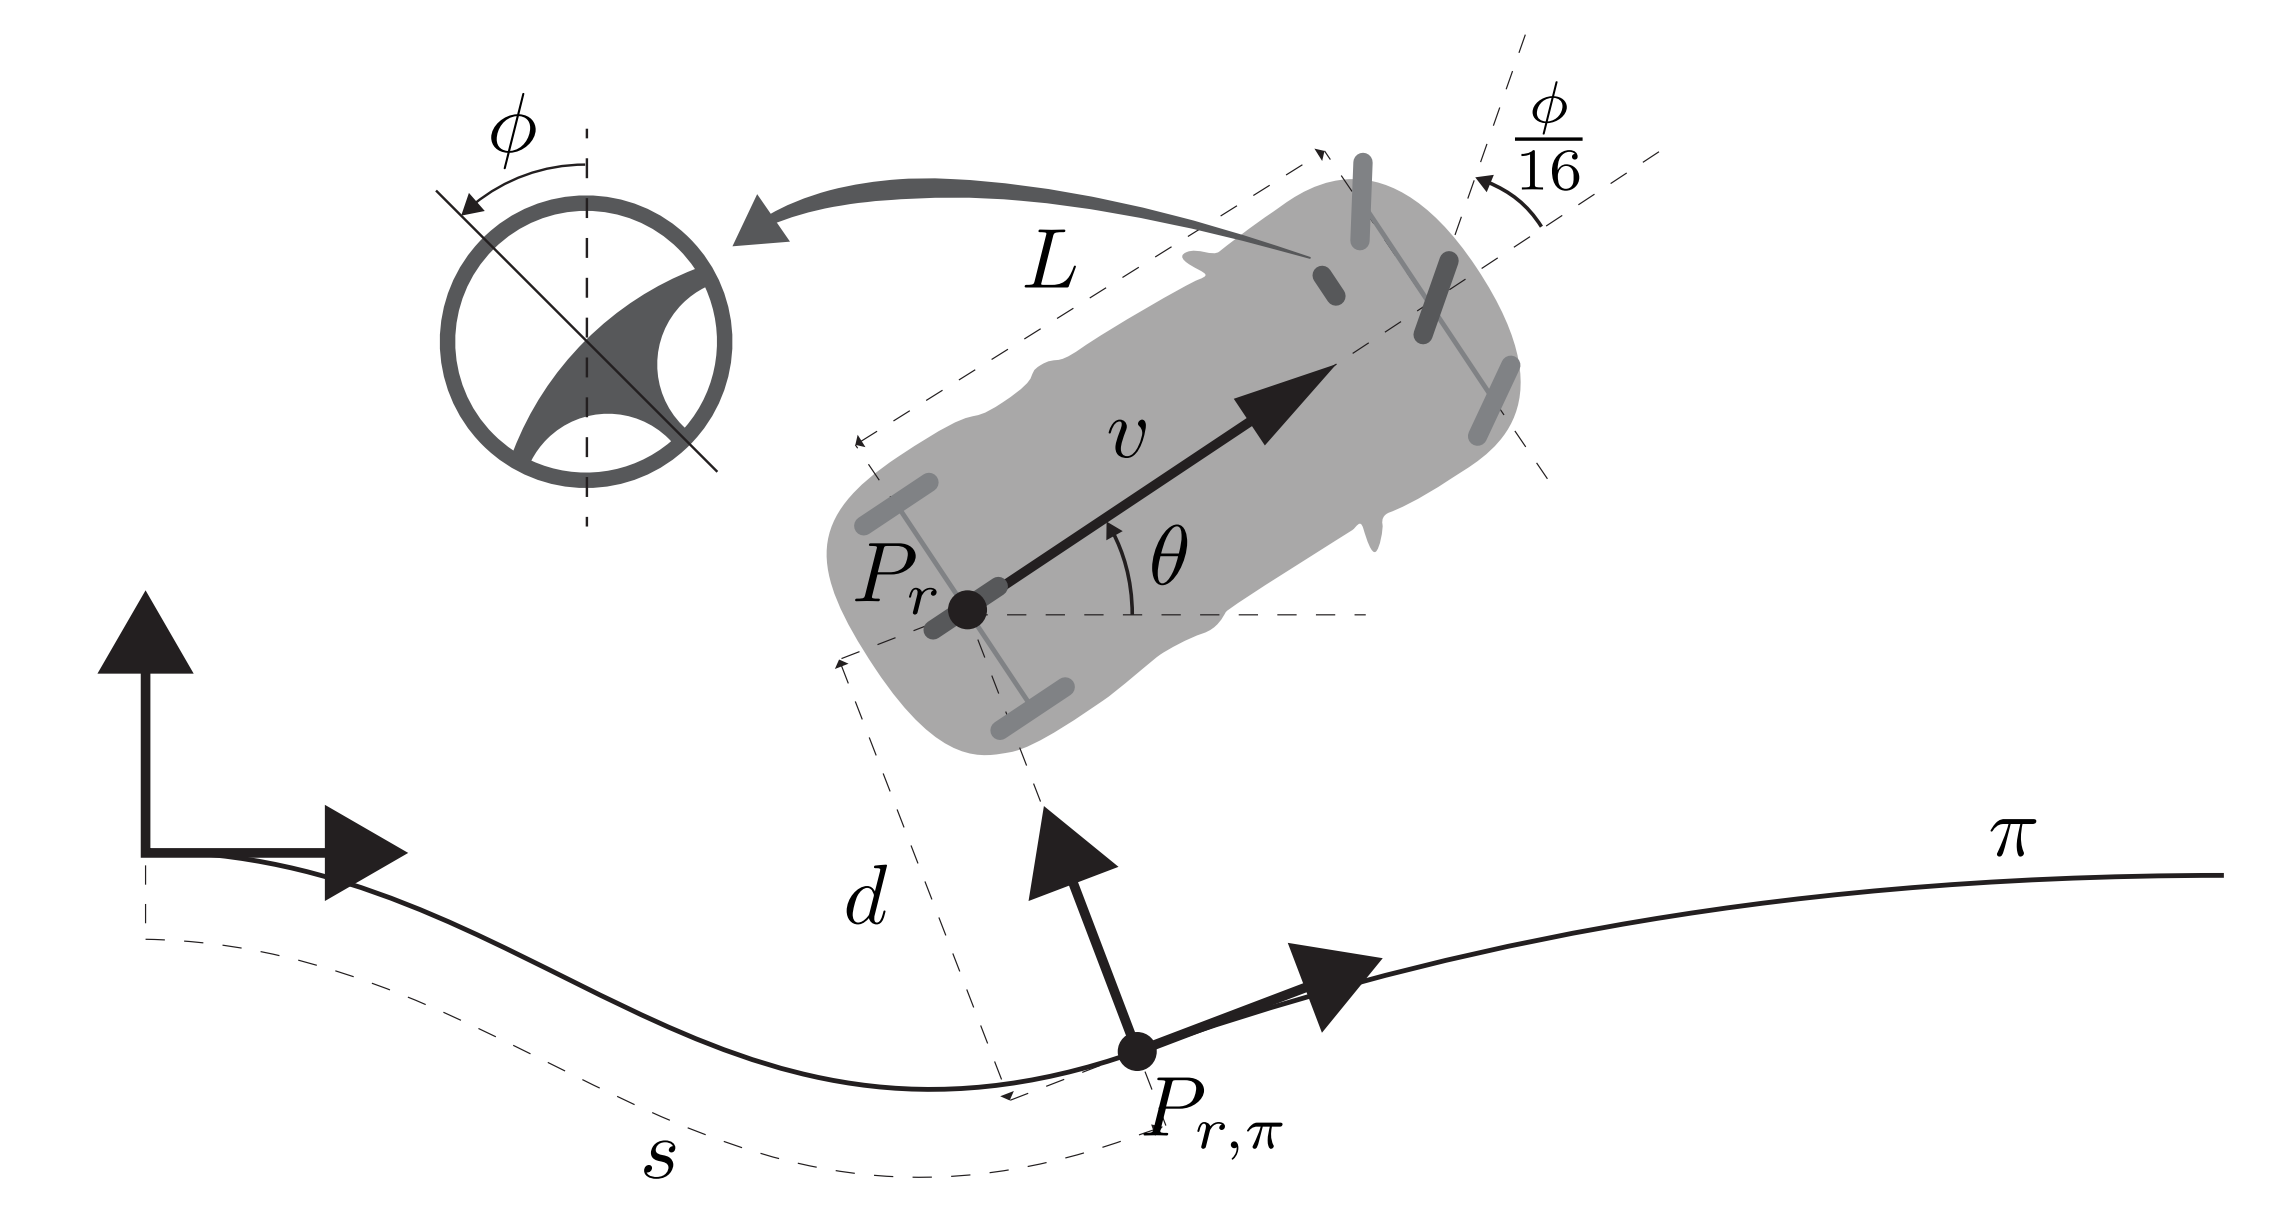
\includegraphics[width=0.6\textwidth]{Latex report/image/system_def.png}
    \caption{Coordinate system}
    \label{fig:sys_def}
\end{figure}

\subsubsection*{System's model}
With the variable defined above, one may write the dynamic of the system with the following equations :
\begin{align}
    \dot{s} &= \frac{v \cos(\theta_e)}{1 - d\kappa(s)}\\
    \dot{d} &= v \sin(\theta_e)\\
    \dot{\theta_e} &= \frac{v}{L}\tan(\frac{\phi}{16}) - \kappa(s)\dot{s}\\
    \dot{v} &= \sigma_v (v_{ref} - v)\\
    \dot{\phi} &= \sigma_{ref} (\phi_{ref} - \phi)\\
\end{align}
\\
In the following, state measurement is assumed unless stated otherwise and the states and control input of the system are :
\begin{align}
    \bold{x} &= [x_1, x_2, x_3, x_4, x_5] = [s,d,\theta_e, v, \phi]\\
    \bold{u} &= [u_1, u_2] = [v_{ref}, \phi_{ref}]\\
    \bold{y} &= \bold{x}
\end{align}


\subsection{Questions}
\subsubsection*{Question 0.1 : Rewrite the non-linear model in the standart form $\bold{\dot{x}} = f(\bold{x}, \bold{u})$}
\begin{equation}
    \left[ {\begin{array}{c}
        \dot{x}_1\\
        \dot{x}_2\\
        \dot{x}_3\\
        \dot{x}_4\\
        \dot{x}_5\\
    \end{array} } \right]
    =
    \left[ {\begin{array}{c}
        f_1(x)\\
        f_2(x)\\
        f_3(x)\\
        f_4(x)\\
        f_5(x)\\
    \end{array} } \right] 
    =
    \left[ {\begin{array}{c}
        \frac{x_4 \cos(x_3)}{1 - x_2\kappa(x_1)}\\
        x_4 \sin(x_3)\\
        \frac{x_4}{L}\tan(\frac{x_5}{16}) - \frac{\kappa(x_1) x_4 \cos(x_3)}{1 - x_2 \kappa(x_1)}\\
        \sigma_v (u_1 - x_4)\\
        \sigma_{ref} (u_2 - x_5)\\
    \end{array} } \right]
\end{equation}



\subsubsection*{Question 0.2 : Given the chosen state space, why it wouldn’t be appropriate linearizing the system around a nominal point.}
There are no such point that are good around the whole trajectory.



\subsubsection*{Question 0.3 : Calculate the nominal trajectory representing the constant-speed perfect tracking situation (that is, a situation where the vehicle drives perfectly on the path and at a constant speed $\bold{v_{ref}}$ ) for a path of constant curvature $\bold{\kappa_{ref}}$.}
Several assumption are made that implies the following :
\begin{itemize}
    \item Constant path curvature : $\kappa(s) \longrightarrow \kappa_{ref}$
    \item Constant speed : $v(s) \longrightarrow v_{ref}$
    \item Vehicle drives perfectly on the the path $\longrightarrow$ no error and no error dynamics ($d=0, \dot{d}=0, \theta_e=0, \dot{\theta_e}=0$)
\end{itemize}
Thus, we already know $\bar{x}_2(t) = 0$, $\bar{x}_3(t) = 0$, $\bar{x}_4 = u_1$. In order to find $\Bar{x}_1(t)$, one can substitute the known variable in $f_1(x)$

\begin{equation}\begin{align}
    \dot{\Bar{x}}_1(t) =  \frac{\bar{x}_4 \cos(\bar{x}_3)}{1 - \bar{x}_2\kappa(s)}
        =v_{ref} = u_1  
\end{align} \end{equation}
By integration, one may find :
\begin{equation}
    \Bar{x}_1(t) = u_1 t + s_0
\end{equation}
\\
Moreover, to find $\bar{x}_5(t)$,  one may want to use $f_3(t)$ and substitute with the known variable.
\begin{equation}\begin{align}
    \dot{\bar{x}}_3 &= f_3(\bar{x}) =
    \frac{\bar{x}_4}{L}\tan\left(\frac{\bar{x}_5}{16}\right) - \frac{\kappa(\bar{x}_1) \bar{x}_4 \cos(\bar{x}_3)}{1 - x_2 \kappa(\bar{x}_1)} \iff\\
    0 &= \frac{v_{ref}}{L}\tan\left(\frac{\bar{x}_5}{16}\right) - \kappa_{ref}v_{ref} \iff\\
    \bar{x}_5 &= 16\tan^{-1}\left(\kappa_{ref}L\right)
\end{align}\end{equation}
\\
 Finally, one can write the nominal trajectory as :
\begin{equation}
    \bar{x}
    =
    \left[ {\begin{array}{c}
        \bar{x}_1(t)\\
        \bar{x}_2(t)\\
        \bar{x}_3(t)\\
        \bar{x}_4(t)\\
        \bar{x}_5(t)\\
    \end{array} } \right]
    =
    \left[ {\begin{array}{c}
        u_1 t + s_0\\
        0\\
        0\\
        u_1\\
        16 \tan^{-1}(\kappa_{ref} L)\\
    \end{array} } \right]
    \label{eq:trajectory}
\end{equation}



\subsubsection*{Question 0.4 : Linearize the system around such a nominal trajectory.}
In this part, we will introduce the linearized model of the system. The linearization is done around a point, or in our case, around a trajectory (equation \ref{eq:trajectory}) and for this purpose, we will introduce the small signal linearization, which is the deviation of the state from an nominal point/trajectory.\\
\\
Small signal linerization :
\begin{equation}
    \begin{align}
        \Tilde{x} &= x - \Bar{x}\\
        \Tilde{y} &= y - \Bar{y}\\
        \Tilde{u} &= u - \Bar{u}  
    \end{align}
\end{equation}

Starting from there, the first step is to find the matrices $A$ and $B$ of the linear system using the first order Taylor expansion of the non-linear model.
\begin{align}
    A &= 
    \left[ {\begin{array}{cccc}
        \frac{\partial f_1}{\partial x_1} & \frac{\partial f_1}{\partial x_2} & \cdots & \frac{\partial f_1}{\partial x_n}\\
        \frac{\partial f_2}{\partial x_1} & \frac{\partial f_2}{\partial x_2} & \cdots & \frac{\partial f_2}{\partial x_n}\\
        \vdots & \vdots & \ddots & \vdots\\
        \frac{\partial f_n}{\partial x_1} & \frac{\partial f_n}{\partial x_2} & \cdots & \frac{\partial f_n}{\partial x_n}\\
    \end{array} } \right] = 
    \left[ {\begin{array}{ccccc}
        0 &\frac{\kappa_{ref} x_4 \cos(x_3)}{(1 -x_2\kappa_{ref})^2} &\frac{-x_4 \sin(x_3)}{1-x_2\kappa_{ref}} &\frac{\cos(x_2)}{1 - x_2 \kappa_{ref}} &0 \\
        0 &0 &x_4 \cos(x_3) &\sin(x_3) &0\\
        0 &\frac{-\kappa_{ref}^2 x_4 \cos(x_3)}{(1 - x_2\kappa_{ref})^2} &\frac{\kappa_{ref}x_4 \sin(x_3)}{1 - x_2\kappa_{ref}} &\frac{\tan(\frac{x_5}{16})}{L} - \frac{\kapp_{ref} \cos(x_3)}{1 - x_2 \kappa_{ref}} & \frac{x_4}{16 L\cos(\frac{x_5}{16})^2}\\
        0 &0 &0 &-\sigma_v &0\\
        0 &0 &0 &0 &-\sigma_{\phi}
    \end{array} } \right]
\end{align}
\begin{align}
    B &= 
    \left[ {\begin{array}{cc}
        \frac{\partial f_1}{\partial u_1} & \frac{\partial f_1}{\partial u_2}\\
        \frac{\partial f_2}{\partial u_1} & \frac{\partial f_2}{\partial u_2}\\
        \vdots & \vdots \\
        \frac{\partial f_n}{\partial u_1} & \frac{\partial f_n}{\partial u_2}\\
    \end{array} } \right]
    = 
    \left[ {\begin{array}{cc}
        0 &0\\
        0 &0\\
        0 &0\\
        \sigma_v &0\\
        0 &\sigma_{\phi}\\
    \end{array} } \right]
\end{align}

In a second step, one may evaluate this expansion around the reference trajectory $\Bar{x}$ in order to find the matrices $\bar{A}$ and $\bar{B}$.\\
\begin{align}
    \bar{A} &= 
    \left[ {\begin{array}{ccccc}
        0 &\kappa_{ref} v_{ref} &0 &1 &0 \\
        0 &0 &v_{ref} &0 &0\\
        0 &-\kappa_{ref}^2 v_{ref} &0 &0 &\frac{v_{ref}}{16L \cos(\tan^{-1}(\kappa_{ref} L))^2}\\
        0 &0 &0 &-\sigma_v &0\\
        0 &0 &0 &0 &-\sigma_{\phi}
    \end{array} } \right]
\end{align}
\begin{equation}
    \bar{B} = B
\end{equation}

Finally, because state measurement is assumed, $C$ is simply the identity matrix, while $D = 0$. The system can thus be written as : 
\begin{align}
    \dot{\Tilde{x}} &= \Bar{A}\Tilde{x} + \Bar{B}\Tilde{u}\\
    \Tilde{y} &= \Tilde{x}
\end{align}


\subsubsection*{Question 0.5 : Discretize the system using Euler approximation.}
With the small signal linear system found previously, one may want to discretize the system. The following formulation uses the euler approximation :\\

\begin{equation}\begin{align}
    \Tilde{x}(k+1) &= \Tilde{x}(k) + \Delta t \Bar{A}\Tilde{x}(k) + \Bar{B}\Tilde{u}\\
    &= \underbrace{\left(I + \Delta t \Bar{A}\right)}_{\Phi} \Tilde{x}(k) + \underbrace{\Delta t \Bar{B}}_{\Gamma}\Tilde{u}(k)\\
    &= \Phi \Tilde{x}(k) + \Gamma \Tilde{u}(k)
\end{align}\end{equation}
\\
One may know compute the discretize state space matrix $\Phi$ and $\Gamma$, with $\Delta t$ equal to one sampling period $\tau_s$ :

\begin{equation}
    \Phi 
    =
    I + \Delta t \Bar{A}
    =
    \left[ {\begin{array}{ccccc}
        1 &\kappa_{ref} v_{ref}\tau_s &0 &\tau_s &0 \\
        0 &1 &v_{ref}\tau_s &0 &0\\
        0 &-\kappa_{ref}^2 v_{ref}\tau_s &1 &0 &\frac{v_{ref}\tau_s}{16L \cos(\tan^{-1}(\kappa_{ref} L))^2}\\
        0 &0 &0 &1-\sigma_v \tau_s&0\\
        0 &0 &0 &0 &1-\sigma_{\phi}\tau_s
    \end{array} } \right]
\end{equation}

\begin{equation}
    \Gamma 
    =
    \Delta t \Bar{B}
    =
    \left[ {\begin{array}{cc}
        0 &0\\
        0 &0\\
        0 &0\\
        \sigma_v \tau_s &0\\
        0 &\sigma_{\phi} \tau_s\\
    \end{array} } \right]
\end{equation}


